\documentclass[11pt]{article}
\usepackage{goldsteinnotes}
\usepackage{cancel}

\graphicspath{{figures/}}

\newcommand{\Veff}{V_{\textsc{eff}}}
\newcommand{\ut}{\tilde u}

\title{Chapter 3 --- Motion in Central Potential $V(r)$;\\ the Kepler Problem}
\author{HC 6001 \quad--\quad Dr.\ Castillo}
\date{15 October 2024}

\raggedbottom

\begin{document}
\maketitle

\section*{Chapter 3 --- Motion in central potential \texorpdfstring{$V(r)$}{V(r)}}

\[
\vect{L} = \mu r^{2}\dot\phi\,\unit{z}
\qquad
\vect{r} = r\,\unit{r}
\qquad
\vect{p} = \mu\,\dot{\vect{r}}
\]
\[
\vect{L} = \text{const.\ of motion}
\]
\[
L = T - V = \frac{\mu}{2}\bigl(\dot r^{2} + r^{2}\dot\phi^{2}\bigr) - V(r)
\]
\[
\phi\ \text{cyclic}
\iff \pd{L}{\phi} = 0
\;\Longrightarrow\;
p_{\phi} = \pd{L}{\dot\phi} = \mu r^{2}\dot\phi \equiv \ell
\qquad \text{\textsc{conserved}}
\]
\[
\Veff(r) = V(r) + \frac{\ell^{2}}{2\mu r^{2}}
\]
\[
E = T + V = \frac{\mu}{2}\bigl(\dot r^{2} + r^{2}\dot\phi^{2}\bigr) + V(r)
  = \frac{\mu}{2}\dot r^{2} + \Veff(r)
\]

\subsection*{Universal method \texorpdfstring{$\Rightarrow$}{=>} complete solution}

\[
\boxeq{\;
\begin{aligned}
t &= \int_{r_{0}}^{r}
   \frac{\d r'}{\sqrt{\dfrac{2}{\mu}\left(E - V(r') - \dfrac{\ell^{2}}{2\mu r'^{2}}\right)}}\\[10pt]
\phi &= \phi_{0} + \int_{r}^{t} \frac{\ell}{\mu r^{2}(t')}\,\d t'
\end{aligned}\;}
\qquad
\begin{aligned}
&t = t(r)\\[24pt]
&\phi = \phi(t)
\end{aligned}
\]

\begin{remark}[on the second quadrature]
The lower limit of the $t'$-integral is written on the board with the lecturer's
$\Gamma$-shaped $r$, not with his crossed $t$; it is reproduced here as written.
The differential is cramped and reads at first glance as ``$\!At'$'': it is $\d t'$.
\end{remark}

\noindent Left-hand side of the radial equation, in the variable $u$:
\[
\mu\ddot r
 = -\frac{\ell^{2}}{\mu}\,\frac{1}{r^{2}}\,\dd{}{\phi}\dd{u}{\phi}
 = -\frac{\ell^{2}}{\mu}\,u^{2}\,\ddn{u}{\phi}{2}
\]

\section*{Diff.\ eqn.\ for \texorpdfstring{$r = r(\phi)$}{r = r(phi)}}

\[
\ell = \mu r^{2}\dot\phi
\;\Longrightarrow\;
\dot\phi = \frac{\ell}{\mu r^{2}} = \dd{\phi}{t}
\]
\[
\dd{r}{t} = \dd{r}{\phi}\,\dd{\phi}{t} = \frac{\ell}{\mu r^{2}}\,\dd{r}{\phi}
\]

\begin{figure}[htbp]
\centering
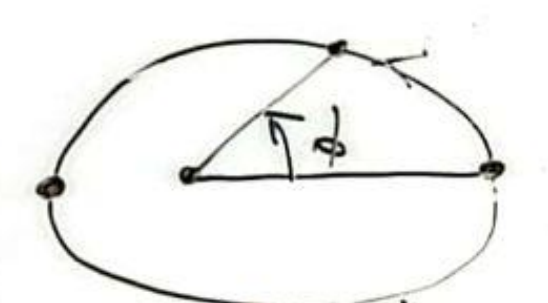
\includegraphics[width=0.46\textwidth]{cp_fig1_orbit_phi.png}
\caption{The orbit and the polar angle $\phi$ measured from the focus.}
\label{fig:orbitphi}
\end{figure}

\subsection*{Radial eq.\ of motion}

\[
\mu\ddot r = -\pd{\Veff}{r}
 = -\pd{}{r}\left(V(r) + \frac{\ell^{2}}{2\mu r^{2}}\right)
\]
\[
\mu\ddot r = F(r) + \frac{\ell^{2}}{\mu r^{3}}
\qquad\qquad
\pd{}{r}\bigl(r^{-2}\bigr) = (-2)\,r^{-3}
\]
\[
u = \frac{1}{r},
\qquad
\dd{u}{\phi} = \dd{u}{r}\,\dd{r}{\phi} = \frac{-1}{r^{2}}\,\dd{r}{\phi}
\]
\[
\frac{\ell^{2}}{\mu r^{3}} = \frac{\ell^{2}}{\mu}\,u^{3}
\;\Longrightarrow\;
\text{RHS:}\quad F\!\left(\tfrac{1}{u}\right) + \frac{\ell^{2}}{\mu}\,u^{3}
\]
\[
\text{LHS:}\quad
\mu\,\ddt{}\dd{r}{t}
 = \mu\,\ddt{}\,\frac{\ell}{\mu r^{2}}\,\dd{r}{\phi}
 = \cancel{\mu}\,\frac{\ell}{\cancel{\mu}\,r^{2}}\,\dd{}{\phi}
   \left(\frac{\ell}{\mu r^{2}}\,\dd{r}{\phi}\right)
\]

\noindent $\underline{\text{LHS} = \text{RHS}}$:
\[
\boxeq{\;
-\frac{\ell^{2}}{\mu}\,u^{2}\,\ddn{u}{\phi}{2}
 = F\!\left(\tfrac{1}{u}\right) + \frac{\ell^{2}}{\mu}\,u^{3}
\;}
\qquad
\begin{aligned}
&\textsc{generic eq.\ of trajectory}\\
&\textsc{for arbitrary } V(r)
\end{aligned}
\]

\begin{remark}[exponents]
The two powers of $u$ in the boxed line differ: $u^{2}$ multiplies
$\d^{2}u/\d\phi^{2}$ on the left, $u^{3}$ stands alone on the right. The two
glyphs are nearly identical at board scale; the left-hand power is fixed
independently by the chain $\mu\ddot r = -(\ell^{2}/\mu)u^{2}\,\d^{2}u/\d\phi^{2}$
recorded above.
\end{remark}

\section*{Eq.\ for trajectory \texorpdfstring{$r(\phi)$}{r(phi)}}

\[
F(r) = -\pd{V}{r}
\]
\[
\dd{V}{r} = \dd{V}{u}\,\dd{u}{r} = -u^{2}\,\dd{V}{u},
\qquad
\dd{u}{r} = -\frac{1}{r^{2}} = -u^{2}
\]
\[
F\!\left(\tfrac{1}{u}\right) = F(r) = -\dd{V}{r} = u^{2}\,\dd{V(1/u)}{u}
\]

\noindent The next line is struck out on the board --- a superseded intermediate
step, kept here as retracted:
\begin{center}
\retracted{$-F(1/u) = -u^{2}\,\d V(1/u)/\d u$}\retractednote
\end{center}

\[
-F\!\left(\tfrac{1}{u}\right)
 = \frac{\ell^{2}}{\mu}\,u^{2}\left[\,u + \ddn{u}{\phi}{2}\,\right]
\]
\[
-\cancel{u^{2}}\,\dd{V}{u}
 = \frac{\ell^{2}}{\mu}\,\cancel{u^{2}}\left[\,u + \ddn{u}{\phi}{2}\,\right]
\]

\noindent The two struck factors $u^{2}$ cancel, leaving
\[
\boxeq{\;
\ddn{u}{\phi}{2} + u = -\frac{\mu}{\ell^{2}}\,\dd{}{u}V\!\left(\tfrac{1}{u}\right)
\;}
\qquad
\begin{aligned}
&\textsc{eq.\ for trajectory } r(\phi)\\
&\text{solve for given } V
\end{aligned}
\]
\[
u = u_{0}\ \text{ for }\ \phi = \phi_{0},
\qquad
\dd{u}{\phi} = 0
\]
\[
\dd{u}{\phi} = 0 \iff \text{max.\ or min.\ } r \text{ point}
\]

\begin{remark}[a slip in the second derivative]
In the line $-F(1/u) = (\ell^{2}/\mu)u^{2}[\,u + \d^{2}u/\d\phi^{2}\,]$ the
superscript $2$ on the numerator $\d$ is written detached and set high above the
fraction, so that the term can be misread as $\d u/\d\phi^{2}$. It is written
correctly and tightly on the line immediately below; both are read here as
$\d^{2}u/\d\phi^{2}$.
\end{remark}

\section*{Gravitation case --- Kepler problem}

\begin{remark}[ink]
\textsc{gravitation case} is written in green on the board; \textsc{kepler
problem}, underlined, is in blue.
\end{remark}

\[
V = -\frac{k}{r} = -k u,
\qquad
\dd{V}{u} = -k
\]
\[
\boxeq{\;\ddn{u}{\phi}{2} + u = \frac{k\mu}{\ell^{2}}\;}
\qquad
\begin{aligned}
&\text{harmonic oscillator}\\
&\text{with shifted origin}
\end{aligned}
\]

\begin{aside}
\[
\ut = u - \frac{k\mu}{\ell^{2}}
\qquad\Longrightarrow\qquad
\boxeq{\;\ddn{\ut}{\phi}{2} + \ut = 0\;}
\]
\emph{Homogeneous solution}\footnote{The word \textsc{solution} runs into the
board frame in the photograph and its last letters are obscured on the board
itself.}
\begin{align*}
\ut(\phi)   &= A\cos(\phi - \phi_{0}),\\
\ut{}'(\phi)  &= -A\sin(\phi - \phi_{0}),\\
\ut{}''(\phi) &= -A\cos(\phi - \phi_{0}) = -\ut(\phi).
\end{align*}
\end{aside}

\[
\boxeq{\;
u(\phi) = \frac{k\mu}{\ell^{2}} + A\cos(\phi - \phi_{0})
\;}
\]

\begin{figure}[htbp]
\centering
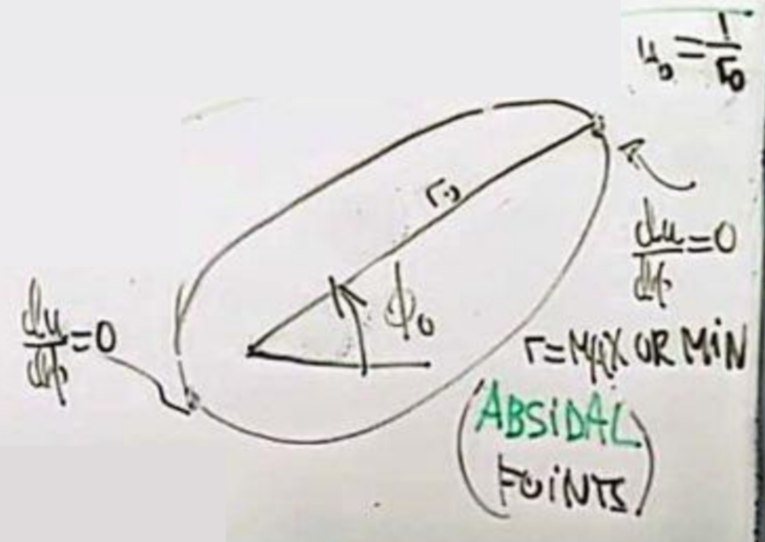
\includegraphics[width=0.50\textwidth]{cp_fig2_apsidal.png}
\caption{Apsidal points of the orbit: $u_{0} = 1/r_{0}$, and
$\d u/\d\phi = 0$ at both ends of the major axis, where $r$ is a maximum or a
minimum. The board's spelling \textsc{absidal} is reproduced verbatim
[editorial note: the standard spelling is \emph{apsidal}]; the parenthesis
\textsc{(absidal points)} is written in green.}
\label{fig:apsidal}
\end{figure}

\[
\boxeq{\;
u(\phi) = \frac{k\mu}{\ell^{2}}\Bigl[\,e\cos(\phi - \phi_{0}) + 1\,\Bigr]
        = \frac{1}{r}
\;}
\]
\[
e\ \text{constant},
\qquad
e \equiv \frac{A}{\,k\mu/\ell^{2}\,}
\]

\subsection*{Using the universal method}

\[
u'' = -u + \frac{k\mu}{\ell^{2}}
\qquad
\Downarrow \times\, u'(\phi)
\]
\[
\dd{u}{\phi} = \bigl(u'\bigr)^{2} = \sqrt{\phantom{1 + \frac{2\ell^{2}E}{\mu k^{2}}}}
\]

\begin{caveat}
The radical on this line is drawn in full --- stroke and vinculum --- but its
interior was \underline{left empty} on the board: it contains only a stray dot
and a short dash, no expression. Nothing is supplied here. Note also that, as
written, $\d u/\d\phi = (u')^{2}$ is loose notation, since $u'$ \emph{is}
$\d u/\d\phi$; the object intended is the first integral obtained by multiplying
through by $u'(\phi)$. Transcribed as written.
\end{caveat}

\[
\d\phi = \frac{\d u}{u'}
\]
\[
\vdots
\]

\noindent A vertical dotted ellipsis of about six dots runs from the line above
down to the boxed result; the elided steps are not reconstructed here.

\[
\boxeq{\;
u = \frac{\mu k}{\ell^{2}}
   \left[\,1 + \sqrt{1 + \frac{2\ell^{2}E}{\mu k^{2}}}\;\cos(\phi - \phi_{0})\,\right]
 = \frac{1}{r}
\;}
\]
\[
\boxeq{\;
e \equiv \sqrt{1 + \frac{2\ell^{2}E}{\mu k^{2}}}
\;}
\]

\begin{remark}[scope of the radical]
The vinculum terminates before $\cos(\phi-\phi_{0})$: the cosine stands outside
the square root, consistent with the boxed definition of $e$ on the line below.
\end{remark}

\end{document}
